\chapter{RESULTADOS}
\label{chp:resultados}

Duas aplicações em Python 3.8\footnote{\url{https://docs.python.org/3.8/}} foram criadas e publicadas. O \emph{Ehrpreper}\footnote{\url{https://github.com/ClaudioBorges/ehrpreper}}, contendo a etapa de preparação do conjunto de dados, e o \emph{Erudite}\footnote{\url{https://github.com/ClaudioBorges/ehrudite}}, com o treinamento e testes dos modelos de aprendizado profunda. Devido a sensibilidade das informações, o conjunto de dados \textit{MIMIC-III} não foi incluído no repositório, mas é necessária sua referência para reprodução dos resultados.

\section{AMBIENTE DE DESENVOLVIMENTO}
\label{sec:results-environment}

Os modelos foram treinados, validados e testados em um computador de dois \textit{sockets} Intel\textsuperscript{\textregistered} Xeon\textsuperscript{\textregistered} Gold 5118 com 188 Gigabytes de memória RAM e uma placa de vídeo Nvidia Tesla V100 com 16 Gigabytes usando CUDA versão 11.0. O sistema operacional utilizado foi um Linux CentOS v7.7.

\section{FERRAMENTAS}
\label{sec:results-tools}

Devido ao conjunto de dados \textit{MIMIC-III} v1.4 apresentar as informações em formato tabular, a biblioteca \emph{Pandas}\footnote{\url{https://pandas.pydata.org/}} foi utilizada facilitar a interpretação. A etapa de aprendizagem utilizou o  \emph{Tensorflow}\footnote{\url{https://github.com/tensorflow/tensorflow}} e o \emph{Keras}\footnote{\url{https://keras.io/}} para definir, treinar e testar os modelos de aprendizado profundo. Também foi utilizada a biblioteca  \emph{scikit-learn}\footnote{\url{https://github.com/scikit-learn/scikit-learn}} para geração da validação cruzada \textit{k-fold} e apoio nas métricas de avaliação.

\section{MÉTRICAS DE AVALIAÇÃO}
\label{sec:results-evaluation-metrics}

Duas métricas foram utilizadas para avaliar as predições geradas pelos modelos treinados: a distância de Levenshtein e a medida-F1. Como não há precedência entre os códigos \gls{icd}, isto é, a ordem em que as anotações aparecem na sentença não interfere no desempenho de predição da tarefa, ambas as sentenças, de códigos atuais e preditos, foram pré-processadas antes da avaliação. Independente da métrica, ambas as sentenças, de códigos atuais e preditos, foram separadas em elementos de um arranjo sempre que o caractere de espaço foi encontrado. Eventuais duplicidades foram removidas.

No caso da distância de Levenshtein, os elementos foram ordenados alfabeticamente e o arranjo foi mesclado em uma única sentença, utilizando o caractere de espaço como separador. Como essa é uma medida absoluta, ou seja, uma sentença com poucos caracteres possui um limite superior inferior a uma sentença com mais elementos; foi necessário normalizar o resultado pelo maior comprimento das sequências. O resultado é portanto limitado entre $0$ a $1$, sendo que, quanto menor, menos edições são necessárias e maior a semelhança; quanto maior, mais edições são necessárias e menos semelhante as sequências são. Desse modo, a distância foi calculada para cada par de caracteres da sentença atual e predita e a média aritmética entre todos os exemplos foi calculada. Portanto, um modelo ideal possui distância de Levenshtein mínima, isto é, igual a $0$.

Houve a necessidade de normalizar os arranjos atuais e preditos para terem o mesmo comprimento e distribuição durante o cálculo da medida-F1. Para isso, a cadeia de caracteres \enquote{<inv>} foi utilizada como código inválido. Esse processo possui três etapas, sendo elas: a separação, utilizando o caractere de espaço para encontrar o início e término dos códigos; a ordenação, dispondo esses códigos de forma organizada; e a inserção, adicionando o código inválido. Considerando as sequências atuais e preditas como \enquote{a01 a02 a03} e \enquote{a02 a01 a04}, o processo de separação resulta em \enquote{[a01, a02, a03]} e \enquote{[a02, a01, a04]}. Em sequência, a ordenação produz \enquote{[a01, a02, a03]} e \enquote{[a01, a02, a04]}; finalmente a inserção, produzindo \enquote{[a01, a02, a03, <inv>]} e \enquote{[a01, a02, <inv>, a04]}. Assim, o primeiro e segundo elementos são iguais enquanto o terceiro e quarto diferences. A média da medida-F1 aumenta sempre que códigos iguais são encontrados, e diminui sempre que códigos diferentes ocorrem. Desse modo, um modelo ideal possui medida-F1 máxima, isto é, igual a $1$.

\section{PREPARAÇÃO DOS DADOS}
\label{sec:results-preparation}

Os relatórios de alta do conjunto de dados do MIMIC-III v1.4 foram extraídos antes dos modelos serem treinados e testados. Para isso, a metodologia a seguir foi utilizada: de um total de $27$ arquivos \glspl{csv}, apenas 2 foram utilizados, o NOTEEVENTS e o DIGNOSES\_ICD, sendo o primeiro o conteúdo em forma textual e o segundo os códigos \gls{icd}-9. O conteúdo do arquivo NOTEEVENTS foi unido com o conteúdo do arquivo DIAGNOSES\_ICD resultando em $59,562$ textos em linguagem natural (conteúdo) e $641,557$ anotações em forma de códigos \gls{icd}-9.

O comprimento mínimo do conteúdo foi de $54$ caracteres, e máximo de $55.728$, com um valor médio de $9.621,67$ e um desvio padrão de $5.539,72$. A Figura \ref{fig:metodology-mimicIII_content_density} apresenta a distribuição de probabilidade do comprimento do conteúdo. A quantidade média de anotações por conteúdo  foi de $11,65$ com um desvio padrão de $6,27$, variando de $1$ até $69$. A Figura \ref{fig:metodology-mimicIII_annotation_density} apresenta a distribuição de probabilidade da quantidade de anotações por conteúdo.
\begin{figure}[htbp]
    \centering
    \begin{minipage}{0.49\textwidth}
        \centering
            \caption{Distribuição de probabilidade do comprimento do conteúdo do relatório de alta de paciente do MIMIC-III.}
            \includegraphics[width=\textwidth]{resources/images/metodologia/ehrpreper-characters-per-content-png}
            \smallcaption{Fonte: Autor.}
            \label{fig:metodology-mimicIII_content_density}
    \end{minipage} \hfill
    \begin{minipage}{0.49\textwidth}
        \centering
            \caption{Distribuição de probabilidade das quantidades de anotações por conteúdo do relatório de alta de paciente do MIMIC-III.}
            \includegraphics[width=\textwidth]{resources/images/metodologia/ehrpreper-annotations-per-content-png}
            \smallcaption{Fonte: Autor.}
            \label{fig:metodology-mimicIII_annotation_density}
    \end{minipage}
\end{figure}

Os códigos \gls{icd}-9 foram traduzidos para \gls{icd}-10 usando o mapeamento realizado por \textcite{Butler2007TheIG}. Esse mapeamento contém o relacionamento entre os códigos \gls{icd}-9 e \gls{icd}-10, e para os casos em que o código \gls{icd}-9 não foi encontrado, o termo $unk$ foi utilizado.

Os códigos \gls{icd}-10 foram truncados em três caracteres, representando sua categoria, incluindo o capítulo e o segundo nível. Esse processo foi realizado para reduzir a quantidade de classes distintas e aumentar a quantidade de exemplos para um mesmo código. Resultando em $1,496$ anotações distintas, incluindo o termo $unk$.

Cada anotação apareceu, em média, em $1.509,71$ conteúdos, com um desvio padrão de $428,84$. $104$ anotações apareceram em apenas 1 conteúdo, $500$ em menos de 10 conteúdos, e $1008$ em menos de $100$ conteúdos. Os cinco códigos com maior frequência foram: $I16$ (aparecendo $22,356$ vezes), $I25$ ($16,705$), $E78$ ($15,654$), $I50$ ($15,471$) e $I48$ ($14,889$). O termo $unk$ apareceu em $15,003$ conteúdos.

Os conteúdos e anotações foram separados em quatro \textit{k-folds}. Cada \textit{k-fold} foi submetido ao ciclo completo de \textit{tokenização}, treinamento e testes sendo que $75\%$ dos pares conteúdo-anotações foram utilizados para o treinamento e $25\%$ para os testes. A média dos resultados dos testes entre os \textit{k-folds} foram utilizadas para apresentar os resultados.

\section{TOKENIZADORES}
\label{sec:results-tokenizers}

O \textit{tokenizador} SentencePiece foi treinado usando o modelo Unigrama. A quantidade de \textit{tokens} do vocabulário do conteúdo foi de $16.384$ em todos os \textit{k-folds}, sendo os $17$ primeiros iguais entre eles. O vocabulário das anotações tinha $128$ \textit{tokens}, e assim como o vocabulário do conteúdo, os $17$ primeiros foram os mesmos em todos os \textit{k-folds}.

O número médio de \textit{tokens} por conteúdo foi de $1.980,40$, desvio padrão de $1.144,30$, quantidade máxima de $11.470$ e mínima de $14$. As anotações tinham $22,50$ \textit{tokens} em média, desvio padrão de $11,76$ e quantidades máximas e mínimas de $82$ e $1$, respectivamente. 

Por questões de comparação de resultados, o \textit{tokenizador} WordPiece também foi treinado utilizando um limite superior de $1e7$ e inferior de $10$, $4$ iterações, comprimento máximo do \textit{token} de $50$ e número máximo de caracteres únicos de $1000$. Após o treinamento, o vocabulário do conteúdo tinha $16.062,00$ \textit{tokens} em média e desvio padrão de $12,75$. Os primeiros $91$ \textit{tokens} foram os mesmos em todos os \textit{k-folds}. O vocabulário das anotações tinha, em média, $122,75$ \textit{tokens} e um desvio padrão de $0,43$, sendo os primeiros $41$ \textit{tokens} os mesmos em todos os \textit{k-fold}.  

O número médio de tokens por conteúdo foi de $1.750,79$ com um desvio padrão de $1.045,38$, quantidade máxima de $11.857$ e mínima de $14$. As anotações tinham em média $21,43$ \textit{tokens}, desvio padrão de $11,97$, quantidade máxima de $89$ e mínima de $1$.

A Tabela \ref{table:tokenizer_results} contém as características dos documentos \textit{tokenizados} para ambos os \textit{tokenizadores}, SentencePiece e WordPiece.
\begin{table}[ht!]
    \caption{Características dos documentos \textit{tokenizados}}
    \label{table:tokenizer_results}
    \centering
    \begin{tabular}{
        >{\centering\arraybackslash}m{0.38\textwidth} | >{\centering\arraybackslash}m{0.25\textwidth} | >{\centering\arraybackslash}m{0.25\textwidth}}
        \hline
    .   Métrica & SentencePiece & WordPiece \\ 
        \hline 
        Tamanho médio do vocabulário do conteúdo (desvio padrão) & $16,384.00$ $(0.00)$ & $16,062.00$ $(12.75)$  \\
        \hline
        Número médio de \textit{tokens} por conteúdo (desvio padrão) & $1,980.40$ $(1,144.30)$ & $1,750.79$ $(1,045.38)$ \\
        \hline
        Tamanho médio do vocabulário da sentença de anotações (desvio padrão) & $128.00$ $(0.00)$ & $122.75$ $(0.43)$ \\
        \hline
        Número médio de \textit{tokens} por sentença de anotações (desvio padrão) & $22.50$ $(11.76)$ & $21.43$ $(11.97)$ \\
        \hline
        \end{tabular}
    \smallcaption{Fonte: Autor}
\end{table}

\section{\texorpdfstring{\MakeUppercase{\xfmrxfmr{}}}{}}
\label{sec:results-transformer-transformer}

A arquitetura de \textit{Transformer} utilizada é a descrita na Seção \ref{sec:transformer}, consistindo de dois codificadores em série, dois decodificadores em série e uma camada final. Cada codificador consiste em uma camada de atenção própria multifacetada, com oito cabeças de dimensão $512$ ($d\_model$), seguida por uma rede \gls{ffn} de mesma dimensionalidade. Cada bloco do codificador é seguido por uma conexão residual com taxa de $0,1$ e normalização. Cada codificador é composto por 3 dimensões: tamanho do lote, comprimento da sequência de entrada e $d\_model$. O decodificador é composto por uma atenção própria multifacetada, seguido por uma atenção mascarada multifacetada contra a respectiva camada do codificador e, em seguida, uma rede \gls{ffn}. Os hiperparâmetros usados nos decodificadores foram os mesmos do codificador e sua dimensionalidade de saída é, respectivamente: tamanho do lote, comprimento da sequência alvo e $d\_model$.

Camadas de \textit{embeddings} independentes foram adicionadas em ambos os codificadores e decodificadores com dimensão $d\_model$ e codificador posicional, como descrito por \cite{Vaswani2017Attention}. A última camada, logo após o decodificador, é uma \gls{ffn} com dimensão igual ao vocabulário alvo (de anotações); isto é, tamanho do lote e tamanho do vocabulário alvo. O otimizador utilizado durante o treinamento foi o mesmo do descrito por \cite{Vaswani2017Attention}, o \gls{adam} com \textit{scheduler} personalizado.

O modelo foi treinado por 265 épocas, sendo que cada uma levou aproximadamente $18$ minutos. A evolução da perda da entropia cruzada, utilizada como medida para o treinamento, é apresentada nas Figuras \ref{fig:result_train_loss_xfmr_sentencepiece} e \ref{fig:result_train_loss_xfmr_wordpiece} para o SentencePiece e WordPiece, respectivamente. É possível notar que a entropia cruzada inicial, assim como a final, foram menores no SentencePiece em relação ao WordPiece, e que ambos os casos apresentaram evolução semelhante.
\begin{figure}[htbp]
    \centering
    \begin{minipage}{0.49\textwidth}
        \centering
            \caption{Evolução da perda da entropia cruzada durante o treinamento da configuração \xfmrxfmr{} utilizando SentencePiece.}
            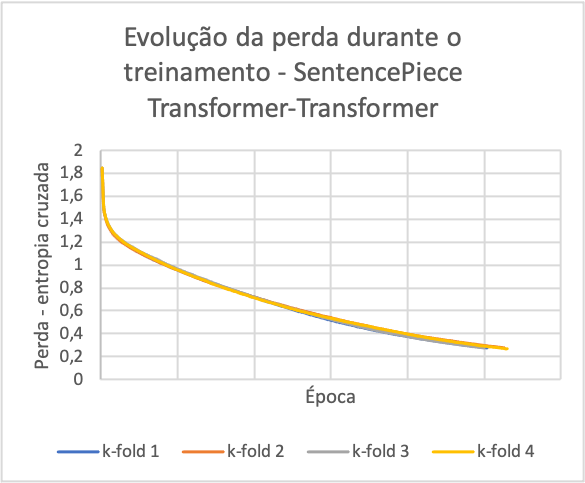
\includegraphics[width=\textwidth]{resources/images/results/result_train_loss_sentencepiece_xfmr_ptbr.png}
            \smallcaption{Fonte: Autor.}
            \label{fig:result_train_loss_xfmr_sentencepiece}
    \end{minipage} \hfill
    \begin{minipage}{0.49\textwidth}
        \centering
            \caption{Evolução da perda da entropia cruzada durante o treinamento da configuração \xfmrxfmr{} utilizando WordPiece.}
            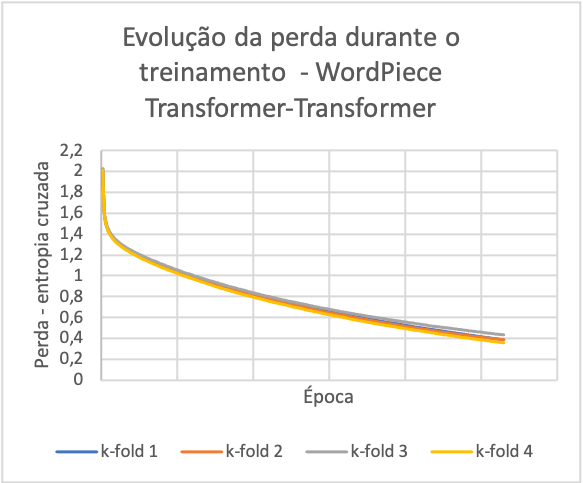
\includegraphics[width=\textwidth]{resources/images/results/result_train_loss_wordpiece_xfmr_ptbr.png}
            \smallcaption{Fonte: Autor.}
            \label{fig:result_train_loss_xfmr_wordpiece}
    \end{minipage}
\end{figure}

O codificador \textit{Transformer} requer um tamanho fixo como entrada, representado por uma sequência de comprimento limitado. Para isso, os \textit{tokens} do conteúdo foram limitados em $2048$ elementos incluindo os \textit{tokens} especiais de início e término de sequência. Casos em que a quantidade de \textit{tokens} foi inferior ao limite, \textit{tokens} de \textit{paddings} foram adicionados. O comprimento da sequência foi definida em $2048$ por ser maior do que o número médio de \textit{tokens}, além de ser possível seu treinamento na placa de vídeo utilizada, conforme Seção \ref{sec:results-environment}. O processo de limitação do conteúdo pode ter impactado a medida-F1 do classificador porque $52,39\%$ dos conteúdos \textit{tokenizados} pelo SentencePiece, e $61,03\%$ através do WordPiece, tiveram sentenças menores ou iguais ao limite utilizado, cooperando com a perda de informação durante o treinamento e teste.

A sequência de anotações não foi limitada, mas \textit{tokens} de \textit{paddings} foram incluídos quando necessário até a posição $128$ além de \textit{tokens} de início e término de sequência.

A Tabela \ref{table:xfmr_xfmr_statistics} apresenta as estatísticas do modelo para ambos os \textit{tokenizadores}. Ela indica que micromédia da medida-F1 do SentencePiece é maior do que a do WordPiece. Porém, tanto a macromédia da medida-F1 quanto a distância de Levenshtein apresentaram resultados piores no SentencePiece. Uma possível explicação para a distância de Levenshtein ser maior no SentencePiece é que foi utilizada a média aritmética, fazendo com que classes infrequentes tenham a mesma importância das classes mais frequentes.
\begin{table}[ht!]
    \caption{Métricas de avaliação do modelo \xfmrxfmr{} utilizando 4 \textit{k-folds}}
    \label{table:xfmr_xfmr_statistics}
    \centering
    \begin{tabular}{
        >{\centering\arraybackslash}m{0.28\textwidth} | >{\centering\arraybackslash}m{0.32\textwidth} | >{\centering\arraybackslash}m{0.28\textwidth}}
        \hline
        Métrica & SentencePiece (desvio padrão) & WordPiece (desvio padrão) \\
        \hline
        Micromédia da medida-F1 & $24,69\% (0,18\%)$ & $23,71\% (0,33\%)$ \\
        \hline
        Macromédia da medida-F1 & $5,03\% (0,05\%)$ & $6,36\% (0,30\%)$ \\
        \hline
        Distância de Levenshtein & $56,25\% (0,37\%)$ & $55,11\% (0,23\%)$ \\
        \hline
    \end{tabular}
    \smallcaption{Fonte: Autor.}
\end{table}

A Tabela \ref{table:xfmr_xfmr_statistics_f1_evolution} apresenta a medida-F1 do modelo \xfmrxfmr{} para os códigos que mais apareceram no conjunto de dados. Em todos os casos a medida-F1 do SentencePiece foi superior ao do WordPiece. As métricas também apresentaram comportamento decrescente quando mais códigos foram adicionados na micromédia, indicando uma degradação na capacidade de classificação.
\begin{table}[ht!]
    \caption{Evolução da micromédia da medida-F1 do modelo \xfmrxfmr{} para os códigos \gls{icd} que mais apareceram no conjunto de dados.}
    \label{table:xfmr_xfmr_statistics_f1_evolution}
    \centering
    \begin{tabular}{
        >{\centering\arraybackslash}m{0.28\textwidth} | >{\centering\arraybackslash}m{0.32\textwidth} | >{\centering\arraybackslash}m{0.28\textwidth}}
        \hline
        Quantidade de códigos que mais apareceram & Micromédia da medida-F1 para o SentencePiece & Micromédia da medida-F1 para o WordPiece \\
        \hline
        10 & $65,54\%$ & $64,44\%$ \\
        \hline
        20 & $61,45\%$ & $60,27\%$ \\
        \hline
        50 & $51,54\%$ & $50,39\%$ \\
        \hline
        100 & $47,60\%$ & $46,58\%$ \\
        \hline
    \end{tabular}
    \smallcaption{Fonte: Autor.}
\end{table}

 A Tabela \ref{table:xfmr_xfmr_statistics_details} apresenta os 20 códigos \gls{icd} com maior medida-F1, para ambos os \textit{tokenizadores} e a porcentagem de vezes que esses códigos apareceram no conjunto de dados. Os códigos $Z38$ e $P07$, que possuem maior medida-F1 se comparado com todos os outros códigos \gls{icd}, obtiveram resultados melhores no WordPiece em relação ao SentencePiece. Os $10$ primeiros códigos obtiveram medida-F1 maior em $7$ casos no WordPiece, enquanto que os $10$ últimos obtiveram medida-F1 maior $7$ casos no SentencePiece, indicando uma tendência da medida-F1 possuir uma distribuição mais uniforme no SentencePiece.
\begin{table}[ht!]
    \caption{As 20 maiores medidas-F1 por código \gls{icd} do transdutor sequencial \xfmrxfmr{} utilizando 4 \textit{k-folds}.}
    \label{table:xfmr_xfmr_statistics_details}
    \centering
    \begin{tabular}{
        >{\centering\arraybackslash}m{0.15\textwidth} | >{\centering\arraybackslash}m{0.19\textwidth} | >{\centering\arraybackslash}m{0.19\textwidth} | >{\centering\arraybackslash}m{0.32\textwidth}}
        \hline
        \gls{icd}-10 & Medida-F1 - SentencePiece & Medida-F1 - WordPiece & Porcentagem de vezes que apareceu no conjunto de dados (valor absoluto)  \\
        \hline
        Z38 & $0,9511$ & $0,9527$ & $0,62\%$ ($3.976$) \\
        \hline
        P07 & $0,9271$ & $0,9346$ & $0,52\%$ ($3.323$) \\
        \hline
        P59 & $0,8321$ & $0,8259$ & $0,45\%$ ($2.864$) \\
        \hline
        Z05 & $0,7801$ & $0,7820$ & $0,43\%$ ($2.757$) \\
        \hline
        I48 & $0,7650$ & $0,7770$ & $2,32\%$ ($14.889$) \\
        \hline
        I25 & $0,7433$ & $0,7444$  & $2,60\%$ ($16.705$) \\
        \hline
        E11 & $0,7360$ & $0,7118$ & $2,16\%$ ($13.887$) \\
        \hline
        P22 & $0,6989$ & $0,7136$ & $0,32\%$ ($2.074$) \\
        \hline
        F20 & $0,7010$ & $0,7115$ & $0,07\%$ ($472$) \\
        \hline
        E03 & $0,7082$ & $0,6139$ & $0,83\%$ ($5.328$) \\
        \hline
        S06 & $0,6818$ & $0,6826$ & $0,42\%$ ($2.722$) \\
        \hline
        I16 & $0,6814$ & $0,6468$ & $3,48\%$ ($22.356$) \\
        \hline
        Z23 & $0,6808$ & $0,6762$ & $0,37\%$ ($2.349$) \\
        \hline
        E78 & $0,6710$ & $0,6486$ & $2,44\%$ ($15.654$) \\
        \hline
        V03 & $0,5717$ & $0,6702$ & $0,04\%$ ($265$) \\
        \hline
        I50 & $0,6600$ & $0,6622$ & $2,41\%$ ($15.471$) \\
        \hline
        J44 & $0,6611$ & $0,6465$ & $1,17\%$ ($7.485$) \\
        \hline
        K50 & $0,6463$ & $0,6368$ & $0,06\%$ ($391$) \\
        \hline
        B20 & $0,6037$ & $0,5433$ & $0,09\%$ ($596$) \\
        \hline
        I21 & $0,5995$ & $0,5857$ & $0,96\%$ ($6.176$) \\
        \hline
    \end{tabular}
    \smallcaption{Fonte: Autor.}
\end{table}

A Figura \ref{fig:result_appears_vs_f1_xfmr_xfmr} apresenta o relacionamento entre a quantidade de vezes que um código \gls{icd}-10 aparece no conjunto de dados e a micromédia da medida-F1 da tarefa de predição. Cada ponto representa uma classe \gls{icd}, as classificações feitas utilizando o WordPiece estão em laranja e o SentencePiece em azul, o eixo vertical utiliza escala logarítmica, enquanto o horizontal linear. Duas linhas de tendência lineares foram adicionadas, a laranja para os dados do WordPiece, e a azul para o SentencePiece. Elas indicam que a medida-F1 possui um relacionamento positivo com a quantidade de vezes de aparecimento; isto é, classes infrequentes tendem a possuir uma medida-F1 menor do que classes que aparecem com maior frequência. Existem casos em que a frequência de uma classe é elevada e sua medida-F1 é baixa, como por exemplo os código $R33$, $T88$ e $K55$, que aparecem em aproximadamente $1000$ exemplos, e apresentaram medida-F1 $0,00\%$ no SentencePiece e $14,59\%$, $7,77\%$, e $19,30\%$ no WordPiece, respectivamente. É interessante notar que tais casos, com número de exemplos igual ou superior a $1000$ e com baixa medida-F1, não foram encontrados no WordPiece, podendo indicar uma tendência de medida-F1 mínima para esse modelo.
\begin{figure}[htbp]
    \centering
        \caption{Relacionamento entre a quantidade de vezes que um código \gls{icd}-10 aparece no conjunto de dados e a micromédia da medida-F1 da tarefa de classificação do modelo \xfmrxfmr{}.}
        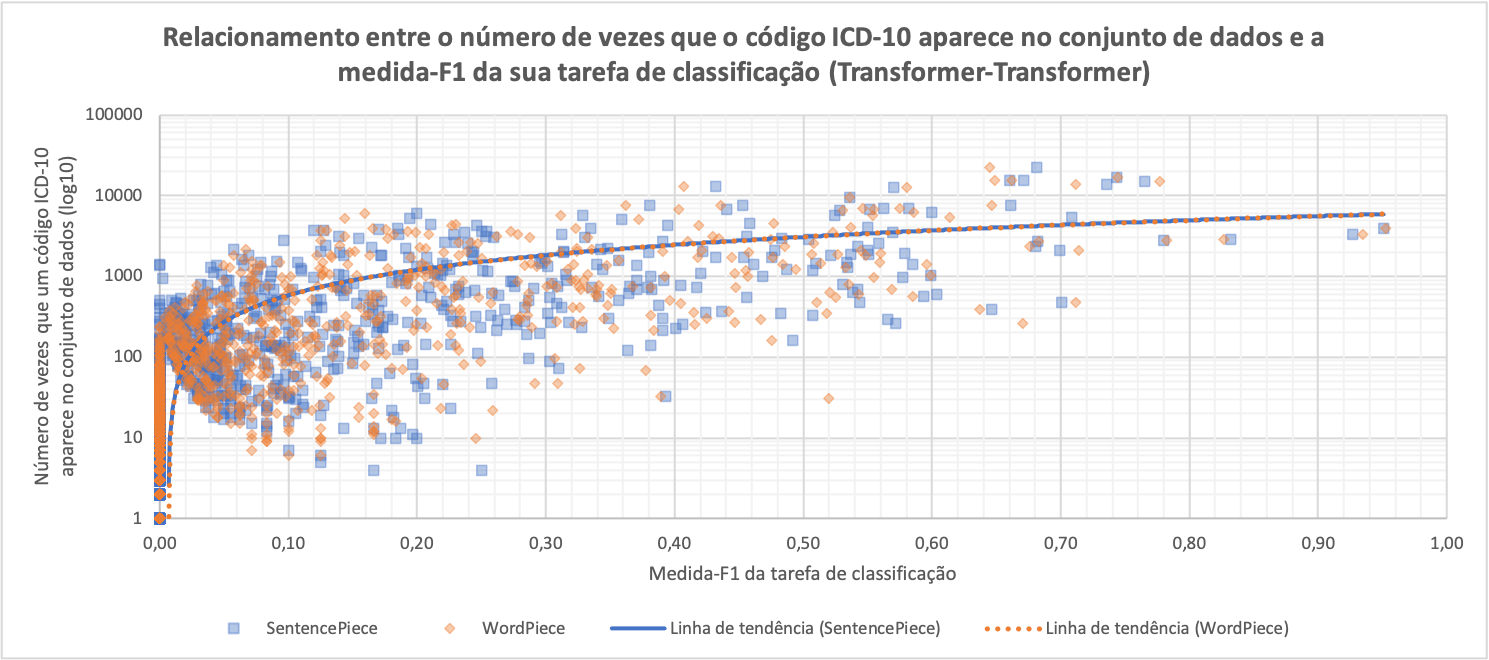
\includegraphics[width=\textwidth]{resources/images/results/result_appears_vs_f1_xfmr_xfmr_log_ptbr.png}
        \smallcaption{Fonte: Autor.}
        \label{fig:result_appears_vs_f1_xfmr_xfmr}
\end{figure}

A Figura \ref{fig:result_f1_range_xfmr} apresenta a distribuição da medida-F1 do modelo para ambos os \textit{tokenizadores}. As barras de cor laranja representam o WordPiece enquanto o azul representa o SentencePiece. Os casos em que a medida-F1 foi zero não foram exibidos para melhorar a visualização ($863$ e $848$ para SentencePiece e WordPiece, respectivamente). O pico da faixa de medida-F1 do SentencePiece ocorre com valores menores que o do WordPiece, corroborando com o resultado inferior da macromédia da medida-F1 para o SentencePiece apresentado anteriormente pela Tabela \ref{table:xfmr_xfmr_statistics}.
\begin{figure}[htbp]
    \centering
        \caption{Distribuição da medida-F1 para o modelo \xfmrxfmr{}.}
        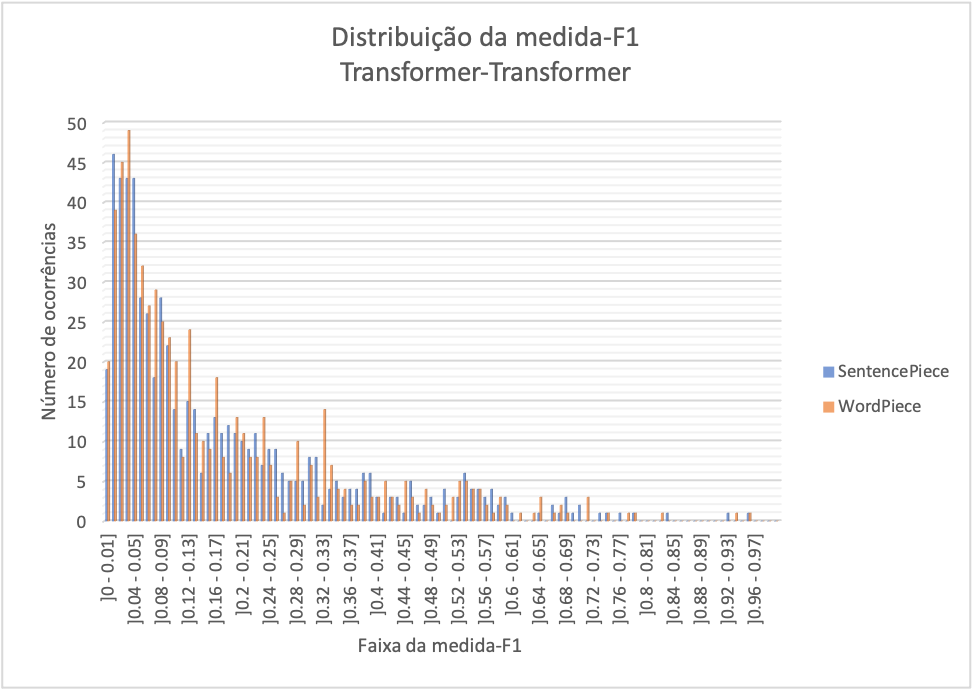
\includegraphics[width=\textwidth]{resources/images/results/result_F1_range_xfmr_ptbr.png}
        \smallcaption{Fonte: Autor.}
        \label{fig:result_f1_range_xfmr}
\end{figure}

Para verificar se a micromédia da medida-F1 do SentencePiece é maior do que a do WordPiece quando aplicado ao modelo de transdução sequencial \xfmrxfmr{}, foi aplicado um teste \textit{t} de \textit{Student}. Considerando $mi_0$ e $S_0$ como os valores da média e da variância da micromédia da medida-F1 do SentencePiece, e $mi_1$ e $S_1$ do WordPiece, a hipótese nula $H_0$ é que $mi_0 = mi_1$ e a hipótese alternativa $H_1$ é $mi_0 <> mi_1$, o teste \textit{t} de \textit{Student} foi realizado e a hipótese nula foi rejeitada com confiança de $99\%$. Desse modo, pode-se afirmar que a utilização do SentencePiece resultou em uma micromédia da medida-F1 superior ao WordPiece.

Um processo semelhante foi realizado com a macromédia da medida-F1 e distância de Levenshtein e, em ambos os casos, a hipótese nula foi rejeitada com confiança de $99\%$, indicando que, a macromédia da medida-F1 do SentencePiece é menor do que a WordPiece, enquanto a distância de Levenshtein do SentencePiece é maior do que a do WordPiece.

\section{\glsentrytext{bi-lstm} - \glsentrytext{lstm} COM ATENÇÃO}
\label{sec:results-bilstm-lstm}

Para fins de comparação entre modelos, uma arquitetura de codificador-decodificador utilizando redes recorrentes também foi investigada. O codificador utilizou uma rede \gls{bi-lstm} e o decodificador uma rede \gls{lstm} com atenção. O codificador foi composto por uma camada de \textit{embedding} com dimensão $512$, seguido por uma camada \gls{bi-lstm} com $64$ unidades escondidas. O resultado de cada \gls{lstm}, isto é, da passagem direta e reversa, foi concatenado, resultando em uma saída de $128$ unidades escondidas.

O estado inicial do decodificador foi definido como ambos, os estados escondido e da célula, do último estágio da forma desenrolada. A primeira camada foi de \textit{embedding} com dimensionalidade $512$, seguida por uma \gls{lstm} com $128$ unidades escondidas. Uma atenção no estilo aditivo de Bahdanau \cite{Bahdanau2016Neural} utilizou a saída do decodificador \gls{lstm} como pergunta sobre a saída do codificador, produzindo os vetores de contexto. Eles então foram concatenados com a saída do decodificador e aplicados a uma camada \gls{ffn} ativada através de uma função $tanh$ gerando os \textit{logits} para os vetores de atenção. Finalmente, os vetores de atenção foram aplicados a uma camada \gls{ffn} com a mesma dimensão do vocabulário de saída.

Para reduzir o tamanho do desenrolamento da rede e limitar o tempo de treinamento, ambas as sequências de entrada e alvo foram truncadas. A sequência de entrada, isto é, os \textit{tokens} do conteúdo, foram truncados em $512$ elementos, incluindo os \textit{tokens} de início e término, além do \textit{padding}, quando necessário. Os \textit{tokens} da sequência de anotação foram truncados em $32$, incluindo os \textit{tokens} de início, término e \textit{padding}. A otimização utilizada para reduzir a quantidade de \textit{tokens} por conteúdo pode ter impactado as métricas da tarefa de classificação. Considerando a quantidade de \textit{tokens} por conteúdo uma distribuição normal com média e desvio padrão conforme a Tabela \ref{table:tokenizer_results}, $10,03\%$ dos conteúdos \textit{tokenizados} pelo SentencePiece, e $11,70\%$ pelo WordPiece, tiveram sentenças menores ou iguais a $512$. No caso das anotações, $79,10\%$ da sequência de anotações \textit{tokenizadas} pelo SentencePiece, e $81,06\%$ pelo WordPiece, tiveram comprimento menor ou igual ao limite utilizado de $32$ \textit{tokens}.

O modelo foi treinado utilizando um otimizador do tipo \Gls{adam} por $15$ épocas para cada um dos $4$ \textit{k-fold}. O tempo de treinamento de cada época foi de aproximadamente duas horas e a evolução da perda da entropia cruzada, utilizada como medida para o treinamento, é apresentada nas Figuras \ref{fig:result_train_loss_lstm_sentencepiece} e \ref{fig:result_train_loss_lstm_wordpiece}. A evolução da entropia cruzada em alguns \textit{k-folds} para o WordPiece apresentou uma instabilidade, em que o valor inicial foi menor do que o valor final; além disso, os \textit{k-folds} não convergiram para um valor específico como apresentado no SentencePiece, em que as quatro execuções aparecem com valores inicial e final semelhantes.
\begin{figure}[htbp]
    \centering
    \begin{minipage}{0.49\textwidth}
        \centering
            \caption{Evolução da perda da entropia cruzada durante o treinamento da configuração \gls{bi-lstm} - \gls{lstm} utilizando SentencePiece.}
            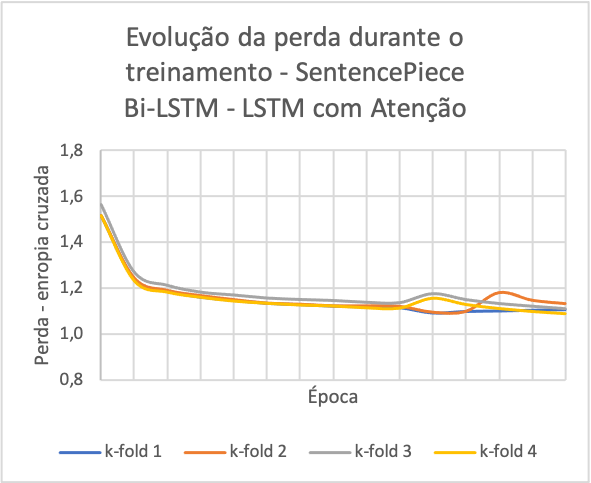
\includegraphics[width=\textwidth]{resources/images/results/result_train_loss_sentencepiece_lstm_ptbr.png}
            \smallcaption{Fonte: Autor.}
            \label{fig:result_train_loss_lstm_sentencepiece}
    \end{minipage} \hfill
    \begin{minipage}{0.49\textwidth}
        \centering
            \caption{Evolução da perda da entropia cruzada durante o treinamento da configuração \gls{bi-lstm} - \gls{lstm} LSTM utilizando WordPiece.}
            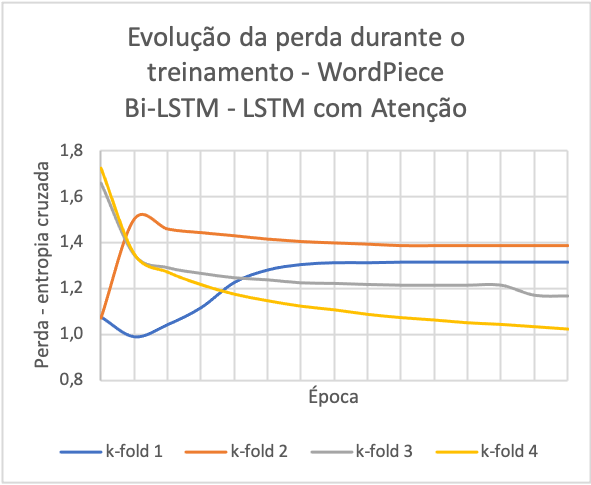
\includegraphics[width=\textwidth]{resources/images/results/result_train_loss_wordpiece_lstm_ptbr.png}
            \smallcaption{Fonte: Autor.}
            \label{fig:result_train_loss_lstm_wordpiece}
    \end{minipage}
\end{figure}

A Tabela \ref{table:lstm_lstm_statistics} apresenta as estatísticas do modelo para ambos os \textit{tokenizadores}. Ela indica que micromédia e a macromédia da medida-F1 do SentencePiece é maior do que a do WordPiece e que a distância de Levenshtein é menor, indicando um melhor desempenho na tarefa de classificação do SentencePiece.
\begin{table}[ht!]
    \caption{Métricas de avaliação do modelo Bi-LSTM - LSTM utilizando 4 \textit{k-folds}}
    \label{table:lstm_lstm_statistics}
    \centering
    \begin{tabular}{
        >{\centering\arraybackslash}m{0.28\textwidth} | >{\centering\arraybackslash}m{0.32\textwidth} | >{\centering\arraybackslash}m{0.28\textwidth}}
        \hline
        Métrica & SentencePiece (desvio padrão) & WordPiece (desvio padrão) \\
        \hline
        Micromédia da medida-F1 & $17,51\% (0,84\%)$ & $13,88\% (2,54\%)$ \\
        \hline
        Macromédia da medida-F1 & $5,70\% (0,60\%)$ & $3,97\% (1,33\%)$ \\
        \hline
        Distância de Levenshtein & $68,14\% (0,71\%)$ & $70,03\% (2,80\%)$ \\
        \hline
        \end{tabular}
    \smallcaption{Fonte: Autor.}
\end{table}

A Tabela \ref{table:lstm_lstm_statistics_f1_evolution} apresenta a medida-F1 do modelo \lstmlstm{} para os códigos que mais apareceram no conjunto de dados. Assim como o modelo \xfmrxfmr{} apresentado na Seção \ref{sec:results-transformer-transformer}, todos os casos a medida-F1 do SentencePiece foi superior ao do WordPiece, e a medida-F1 apresentou comportamento decrescente quando mais códigos foram adicionados na micromédia, indicando uma degradação na capacidade de classificação.
\begin{table}[ht!]
    \caption{Evolução da micromédia da medida-F1 do modelo \lstmlstm{} para os códigos \gls{icd} que mais apareceram no conjunto de dados.}
    \label{table:lstm_lstm_statistics_f1_evolution}
    \centering
    \begin{tabular}{
        >{\centering\arraybackslash}m{0.28\textwidth} | >{\centering\arraybackslash}m{0.32\textwidth} | >{\centering\arraybackslash}m{0.28\textwidth}}
        \hline
        Quantidade de códigos que mais apareceram & Micromédia da medida-F1 para o SentencePiece & Micromédia da medida-F1 para o WordPiece \\
        \hline
        10 & $59,02\%$ & $57,45\%$ \\
        \hline
        20 & $54,05\%$ & $49,28\%$ \\
        \hline
        50 & $44,48\%$ & $39,80\%$ \\
        \hline
        100 & $40,58\%$ & $35,77\%$ \\
        \hline
    \end{tabular}
    \smallcaption{Fonte: Autor.}
\end{table}

A Tabela \ref{table:lstm_lstm_statistics_details} apresenta os 20 códigos \gls{icd} com maior medida-F1, para ambos os \textit{tokenizadores} e a porcentagem de vezes que esses códigos apareceram no conjunto de dados. Diferente do modelo \xfmrxfmr{} apresentado na Seção \ref{sec:results-transformer-transformer}, todos os $20$ códigos apresentaram medida-F1 superior no SentencePiece do que no WordPiece, sendo o código $G20$ teve a maior diferença entre os \textit{tokenizadores}, sendo ela de $31,61\%$.
\begin{table}[ht!]
    \caption{As 20 maiores medidas-F1 por código \gls{icd} do transdutor sequencial \lstmlstm{} utilizando 4 \textit{k-folds}.}
    \label{table:lstm_lstm_statistics_details}
    \centering
    \begin{tabular}{
        >{\centering\arraybackslash}m{0.15\textwidth} | >{\centering\arraybackslash}m{0.19\textwidth} | >{\centering\arraybackslash}m{0.19\textwidth} | >{\centering\arraybackslash}m{0.32\textwidth}}
        \hline
        \gls{icd}-10 & Medida-F1 - SentencePiece & Medida-F1 - WordPiece & Porcentagem de vezes que apareceu no conjunto de dados (valor absoluto) \\
        \hline
        Z38 & $0,9494$ & $0,9206$ & $0,62\%$ ($3.976$) \\
        \hline
        P07 & $0,8917$ & $0,8753$ & $0,52\%$ ($3.323$) \\
        \hline
        P59 & $0,7987$ & $0,7927$ & $0,45\%$ ($2.864$) \\
        \hline
        Z05 & $0,7802$ & $0,7706$ & $0,43\%$ ($2.757$) \\
        \hline
        I25 & $0,7331$ & $0,7266$ & $2,60\%$ ($16.705$) \\  
        \hline
        F20 & $0,6996$ & $0,6931$ & $0,07\%$ ($472$) \\
        \hline
        E11 & $0,6977$ & $0,6705$ & $2,16\%$ ($13.887$) \\
        \hline
        C90 & $0,6933$ & $0,3658$ & $0,03\%$ ($215$) \\ 
        \hline
        J44 & $0,6772$ & $0,4879$ & $1,17\%$ ($7.485$) \\
        \hline
        Z23 & $0,6746$ & $0,6301$ & $0,37\%$ ($2.349$) \\
        \hline
        P22 & $0,6523$ & $0,6482$ & $0,32\%$ ($2.074$) \\
        \hline
        K50 & $0,6498$ & $0,5166$ & $0,06\%$ ($391$) \\
        \hline
        I16 & $0,6470$ & $0,6345$ & $3,48\%$ ($22.356$) \\
        \hline
        E78 & $0,6347$ & $0,5826$ & $2,44\%$ ($15.654$) \\
        \hline
        G20 & $0,6318$ & $0,3157$ & $0,09\%$ ($569$) \\
        \hline
        E10 & $0,5972$ & $0,3879$ & $0,30\%$ ($1.894$) \\
        \hline
        I48 & $0,5935$ & $0,5828$ & $2,32\%$ ($14.889$) \\
        \hline
        C91 & $0,5916$ & $0,3421$ & $0,05\%$ ($293$) \\
        \hline
        G35 & $0,5847$ & $0,2736$ & $0,05\%$ ($333$) \\
        \hline
        E03 & $0,5797$ & $0,4405$ & $0,83\%$ ($5.328$) \\
        \hline
    \end{tabular}
\end{table}

A Figura \ref{fig:result_appears_vs_f1_lstm_lstm} apresenta o relacionamento entre a quantidade de vezes que um código \gls{icd}-10 aparece no conjunto de dados e a micromédia da medida-F1 da tarefa de predição. Assim como o modelo \xfmrxfmr{} apresentado na Seção \ref{sec:results-transformer-transformer}, classes infrequentes tendem a possuir uma medida-F1 menor do que classes que aparecem mais vezes. Os código $N28$ e $Z91$ apareceram aproximadamente $1000$ vezes e sua medida-F1 foi $0,38\%$ e $4,59\%$ para o SentencePiece, e $1,08\%$ e $0,48\%$ para o WordPiece. O código $O08$ apareceu apenas 4 vezes e sua medida-F1 no SentencePiece foi de $25,00\%$, enquanto que no WordPiece ficou com $0,00$, e pode ser considerado um valor atípico. A linha de tendência do WordPiece, em laranja, está ligeiramente acima da linha do SentencePiece, em azul, indicando que a medida-F1 do WordPiece, nessa configuração, tende a aumentar em uma proporção maior, se comparado com o SentencePiece, conforme a quantidade de exemplos de uma classe aumenta.
\begin{figure}[htbp]
    \centering
        \caption{Relacionamento entre a quantidade de vezes que um código \gls{icd}-10 aparece no conjunto de dados e a micromédia da medida-F1 da tarefa de classificação do modelo \lstmlstm{}.}
        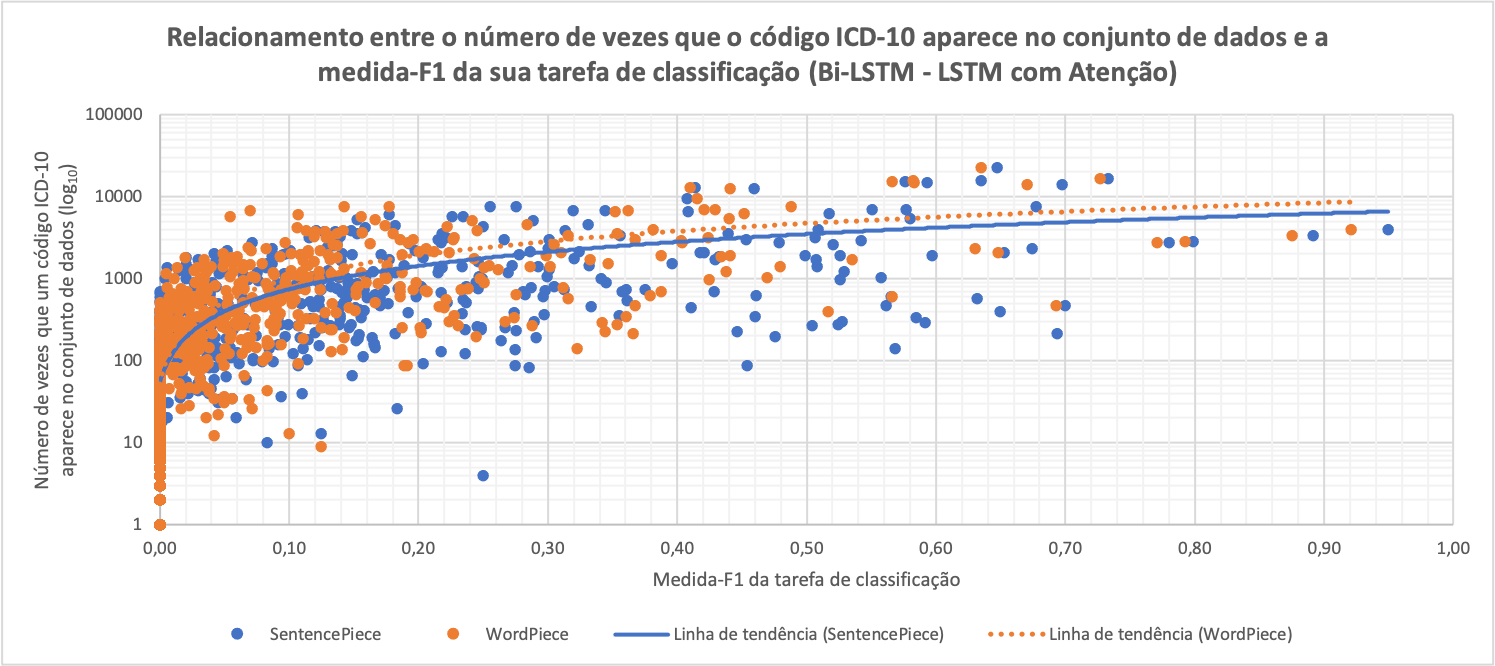
\includegraphics[width=\textwidth]{resources/images/results/result_appears_vs_f1_lstm_lstm_log_ptbr.png}
        \smallcaption{Fonte: Autor.}
        \label{fig:result_appears_vs_f1_lstm_lstm}
\end{figure}

A Figura \ref{fig:result_f1_range_lstm} apresenta a distribuição da medida-F1 do modelo para ambos os \textit{tokenizadores}. As barras de cor laranja representam o WordPiece enquanto o azul representa o SentencePiece. Os casos em que a medida-F1 foi zero foram não foram exibidos para melhorar a visualização ($1030$ e $1037$ para SentencePiece e WordPiece, respectivamente). O pico da faixa de medida-F1 do SentencePiece ocorre com valor ligeiramente menor do que o WordPiece, porém não é suficiente para a macromédia da medida-F1 ser inferior, como ocorreu no modelo \xfmrxfmr{} da Seção \ref{sec:results-transformer-transformer}.
\begin{figure}[htbp]
    \centering
        \caption{Distribuição da medida-F1 para o modelo \lstmlstm{}.}
        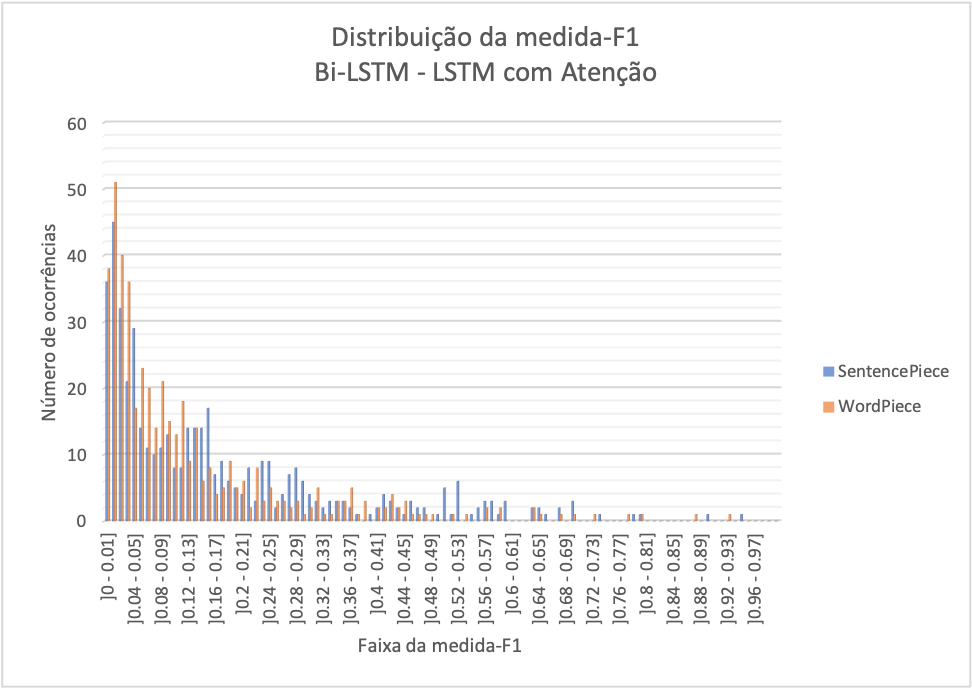
\includegraphics[width=\textwidth]{resources/images/results/result_F1_range_lstm_ptbr.png}
        \smallcaption{Fonte: Autor.}
        \label{fig:result_f1_range_lstm}
\end{figure}

Assim como no modelo \xfmrxfmr{} da Seção \ref{sec:results-transformer-transformer}, o teste \textit{t} de \textit{Student} foi realizado no modelo \lstmlstm{} com hipótese nula de que os valores médios apresentados entre o SentencePiece e o WordPiece da Tabela \ref{table:lstm_lstm_statistics_details} são iguais. O teste mostrou que os valores médios não são os mesmos com confiabilidade de $99\%$, indicando que a micromédia e macromédia da medida-F1 do SentencePiece é maior do que a WordPiece, enquanto a distância de Levenshtein da medida-F1 do SentencePiece é menor do que a WordPiece.

\section{COMPARAÇÃO DOS MODELOS}
\label{sec:results-models-comparison}

Essa Seção compara o modelo \xfmrxfmr{} apresentada na Seção \ref{sec:results-transformer-transformer} e o  \lstmlstm{} da Seção \ref{sec:results-bilstm-lstm}. Todas as comparações foram realizadas utilizando o \textit{tokenizador} SentencePiece por ter apresentado um melhor desempenho.

A Figura \ref{fig:result_appears_vs_f1_lstm_lstm} compara as medidas-F1 de cada código \gls{icd}-10 entre o \xfmrxfmr{} e o \lstmlstm{}. Cada círculo azul representa um código \gls{icd}-10 diferente. A seção laranja contém todos os códigos \gls{icd} em que a medida-F1 do modelo com \textit{Transformer} foi maior do que o modelo com \gls{lstm}, enquanto que a seção cinza contém os códigos em que a medida-F1 do modelo com \gls{lstm} foi maior. De um conjunto de $1,496$ códigos \gls{icd}-10, o \textit{Transformer} apresentou medida-F1 superior em $35.49\%$ enquanto o \gls{lstm} em $8.49\%$. Em todos os outros casos, isto é, $56.02\%$, a medida-F1 foi $0.00\%$.
\begin{figure}[htbp]
    \centering
        \caption{Comparação da medida-F1 para códigos \gls{icd}-10 entre os modelos \xfmrxfmr{} e \lstmlstm{}.}
        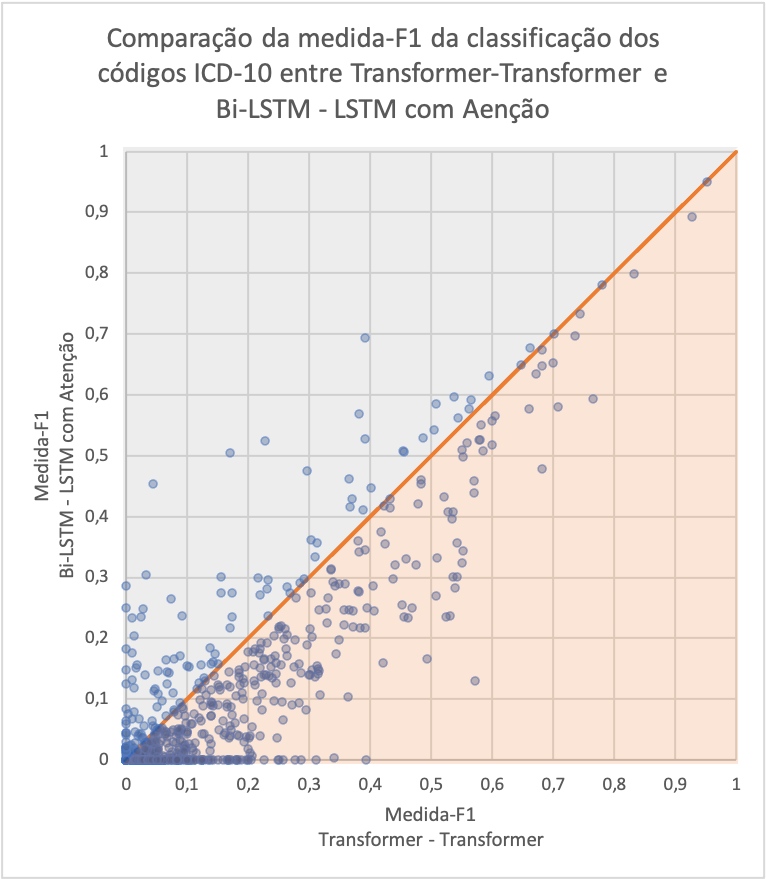
\includegraphics{resources/images/results/result_f1_comparison_xfmr_lstm_ptbr.png}
        \smallcaption{Fonte: Autor.}
        \label{fig:result_f1_comparison_xfmr_lstm}
\end{figure}

Do conjunto de códigos \gls{icd} em que o modelo com \gls{lstm} superou o \textit{Transformer}, os que tiverem maiores diferenças entre as medidas-F1 foram $G80$ (diferença de $41,04\%$), $D86$ ($33,44\%$), $C90$ ($30,28\%$), $F25$ ($29,67\%$), e $G14$ ($28,54\%$). No caso do \textit{Transformer}, os cinco códigos foram: $V03$ (diferença de $44,22\%$), $P90$ ($39,34\%$), $Z89$ ($33,84\%$), $V29$ ($32,66\%$), e $P23$ ($31,04\%$). Os códigos $Z05$, $K64$, $C61$ obtiveram as medidas-F1 mais próximas, sendo elas, $78,01\%$ e $78,02\%$ para o primeiro, $7,89\%$ e $7,87\%$ para o segundo, e $11,63\%$ e $11,60\%$ para o terceiro, respectivamente para \textit{Transformer} e \gls{lstm}. Os quatro códigos com maiores medida-F1 foram os mesmos tanto para o \textit{Transformer} quanto para o \gls{lstm}, sendo eles: $Z38$, $P07$, $P59$, e $Z05$, possuindo respectivos valores $95,11\%$ e $94,94\%$ para o primeiro, $92,71\%$ e $89,17\%$ para o segundo, $83,21\%$ e $79,87\%$ para o terceiro, e $78,01\%$ e $78,02\%$ para o quarto.

A hipótese de que o desempenho da micromédia da medida-F1 do \xfmrxfmr{} (Seção \ref{sec:results-transformer-transformer}) é maior do que a do \lstmlstm{} (Seção \ref{sec:results-bilstm-lstm}) foi verificada através do teste \textit{t} de \textit{Student}. Considerando $mi_0$ e $S_0$ como os valores da média e da variância da micromédia da medida-F1 do \xfmrxfmr{}, e $mi_1$ e $S_1$ do \lstmlstm{}, a hipótese nula $H_0$ $mi_0 = mi_1$ e a hipótese alternativa $H_1$ $mi_0 <> mi_1$, o teste refutou a hipótese nula com $99\%$ de confiabilidade, indicando que as médias dos modelos são distintas e, consequentemente, a média do \xfmrxfmr{} é superior a do \lstmlstm{}, indicando um desempenho de classificação de códigos \gls{icd}-10 superior.

\section{DISCUSSÃO}
\label{sec:results-discussionn}

Quatro diferentes configurações de transdutor sequencial foram investigadas, duas utilizando o \xfmrxfmr{}, e duas com o \lstmlstm{}. Cada uma delas utilizando o \textit{tokenizador} SentencePiece e WordPiece. As investigações utilizaram métricas da micromédia e macromédia da medida-F1 e distância de Levenshtein.

Para ambos pares de codificadores-decodificadores, a micromédia da medida-F1 para o \textit{tokenizador} SentencePiece foi superior a do WordPiece. Tanto o número médio de \textit{tokens} por conteúdo quanto de sentenças de anotações do SentencePiece é superior ao WordPiece, podendo indicar que há uma relação direta entre a quantidade de \textit{tokens} necessária para representar uma sentença e sua influência no desempenho da tarefa de classificação.

Uma possível razão é a de que, quanto maior a quantidade de \textit{tokens}, maior a capacidade do estágio de \textit{embeddings}, presentes na entrada do codificador e do decodificador, representar seus vetores de forma a influenciar  a tarefa específica, já que há um número maior de possíveis combinações. Do mesmo modo, quanto menor a quantidade de \textit{tokens} por sequencia, menor pode ser sua capacidade de representar os \textit{embeddings} influenciando negativamente sua capacidade de classificação.

Uma outra hipótese é que o algoritmo utilizado para gerar o vocabulário e os \textit{tokens} do SentencePiece influenciam positivamente e de forma superior do que o WordPiece na tarefa específica de classificação \gls{icd}. Porém, mesmo que o desempenho do SentencePiece em relação a micromédia da medida-F1 foi superior, a distância de Levenshtein nem sempre foi. No caso do modelo utilizando \gls{lstm}, a distância é menor no SentencePiece, representando um melhor desempenho, enquanto que no modelo utilizando \textit{Transformer} a distância é menor no WordPiece.

Independente do \textit{tokenizador} e da arquitetura de transdução sequencial, a arquitetura está sujeita ao desbalanceamento de classes. Os códigos \gls{icd} que aparecem mais vezes durante o treinamento tendem a apresentar melhores medidas-F1 do que aqueles que aparecem menos vezes. Desse modo, aumentar a quantidade de exemplos apresentados durante o treinamento pode resultar em uma melhora da medida-F1 desses códigos \gls{icd}. Por outro lado, códigos infrequentes, como algumas patologias raras, tendem a apresentar um resultado inferior. Essa tendência pode ser resultado da incapacidade de modelar a linguagem ou uma predisposição do modelo em predizer classes com maiores chances de aparecerem.

O tempo médio para se treinar uma época do modelo que utilizou o \textit{Transformer} foi $85\%$ menor do que para o \gls{lstm}, resultando na capacidade do \textit{Transformer} de ser treinado por mais épocas em um mesmo intervalo de tempo, causando uma tendência de diminuição da perda de entropia cruzada durante o treinamento. O tempo inferior de treinamento do \textit{Transformer} se deve ao fato dele possuir poucas etapas sequenciais em sua arquitetura, por outro lado, o treinamento do \gls{lstm}, e das redes to tipo recursivas, processam cada \textit{token} sequencialmente, sub-utilizando a capacidade de processamento paralelo das placas de vídeos. 

Dos 20 códigos \gls{icd} com maiores medida-F1 para o modelo que utilizou o \textit{Transformer} e para o \gls{lstm}, quinze aparecem para ambas as arquiteturas, sendo que os quatro primeiros códigos são os mesmos e estão dispostos na mesma ordem em ambos os modelos. Porém, a arquitetura \lstmlstm{} apresentou medida-F1 inferior a do \textit{Transformer}.

De modo similar, a micromédia geral da medida-F1 para o \textit{Transformer} também foi superior ao \gls{lstm}, sendo $24,69\%$ e $17,51\%$, respectivamente, indicando um desempenho de classificação superior na configuração do \textit{Transformer} apresentada. A macromédia da medida-F1 foi de $5,03\%$ para o \textit{Transformer} contra $5,70\%$ para o \gls{lstm}, indicando que o \textit{Transformer} está mais sujeito ao desbalanceamento de classes resultando em uma medida-F1 menor para classes infrequentes. A distância de Levenshtein também obteve desempenho superior no \textit{Transformer}, sendo ela $56,25\%$ contra $68,14\%$ no \gls{lstm}, indicando que resultados gerados pelo \gls{lstm} precisam de $21,14\%$ mais inserções, alterações ou deleções do que pelo \textit{Transformer}.

Devido a limitações computacionais, o tamanho máximo do conteúdo do relatório de alta do paciente foi truncado em uma posição diferente entre o \textit{Transformer} e o \gls{lstm}. O primeiro utilizou $2048$ \textit{tokens} enquanto o segundo apenas $512$, sendo que $47,61\%$ dos conteúdos possuem comprimento superior no caso do \textit{Transformer} enquanto $89,97\%$ no caso do \gls{lstm}. Essa diferença significativa de perda de informação, quatro vezes maior no \gls{lstm}, assim como a quantidade inferior de épocas de treinamento, $17$ vezes maior no \textit{Transformer}, podem ter contribuído com a medida-F1 menor no \gls{lstm} em relação ao \textit{Transformer}.

Mesmo que a qualidade de classificação do modelo \xfmrxfmr{} seja superior do que a \lstmlstm{}, isso não representa que essa premissa seja válida independente do código \gls{icd}. Existem situação em que a classificação de certos códigos \gls{icd} realizadas pelo modelo com \gls{lstm} é superior do que o \textit{Transformer}, porém a maioria dos casos o \textit{Transformer} apresentou melhor desempenho.